\documentclass{article}

\usepackage[T2A]{fontenc}
\usepackage[utf8]{inputenc}
\usepackage[russian]{babel}
\usepackage{amsmath}
\usepackage{amssymb}
\usepackage{amsthm}
\usepackage{mathrsfs}
\usepackage{booktabs}

\usepackage{dan2e}

% Эти четыре строчки, чтобы исправить проблему с компиляцией 
% т.к. не определялся if@Russian, возможно из-за более новой версии babel
\makeatletter
\@ifundefined{@Russian}{\newif\if@Russian \@Russiantrue}{}
\@ifundefined{@TVP}     {\newif\if@TVP    \@TVPfalse}{}
\makeatother

\theoremstyle{definition}
\newtheorem{defi}{Определение}
\theoremstyle{plain}
\newtheorem{remark}{Пример}
\newtheorem{theorem}{Теорема}
\newtheorem{OldTheorem}{Теорема}
\renewcommand{\theOldTheorem}{\Alph{OldTheorem}}

\newtheorem{Theorem}{Теорема}
\renewcommand{\theTheorem}{\arabic{theorem}$^\prime$}

\begin{document}

\Volume{505}
\Year{2025}
\Pages{46--49}

\udk{517.54}

\title{Оценка общих и специальных знаний в больших языковых моделях для русского языка посредством воспроизведения энциклопедических статей}

\author{Д.\,А.~Григорьев\Addressmark[1]\Emailmark[1], Д.\,И.~Чернышев\Addressmark[1]\Emailmark[2]}

\Addresstext[1]{Московский государственный университет им.~М.\,В.~Ломоносова, Москва, Россия}

\Emailtext[1]{dagrig14@yandex.ru}

\Emailtext[2]{chdanorbis@yandex.ru}

\markboth{Д.\,А.~Григорьев, Д.\,И.~Чернышев}{Оценка общих и специальных знаний в больших языковых моделях}

\presentedby{Представлено кем-то}

\dateA{16.08.2025}
\dateB{20.08.2025}
\dateC{31.08.2025}

\alttitle{Evaluating general and special knowledge in large language models for Russian language through replication of encyclopedia articles}

\altauthor{D.\,A.~Grigoriev\Addressmark[a]\Emailmark[1], D.\,I.~Chernyshev\Addressmark[a]\Emailmark[2]}

\altAddresstext[a]{Lomonosov Moscow State University, Moscow Center for Fundamental and Applied Mathematics, \\ Moscow, Russian Federation}

\altpresentedby{Presented by Academician of the RAS B.\,S.~Kashin}

\maketitle

\doi{10.31857/S2686954322040117}

\begin{abstract}
В данной работе предложен и реализован бенчмарк WikiBench для оценки аналитических способностей больших языковых моделей при составлении научно-энциклопедических текстов на русском языке. 
\end{abstract}

\begin{keywords}
бенчмарк, Википедия, Рувики, large language model
\end{keywords}

\begin{altabstract}
In this work we propose and implement WikiBench for evaluating the analytical capabilities of large language models in generating scientific and encyclopedic texts in Russian.
\end{altabstract}

\begin{altkeywords}
benchmark, Wikipedia, Ruwiki, large language model
\end{altkeywords}


\section*{Введение}

Современные большие языковые модели демонстрируют впечатляющие результаты в генерации текстов различной стилистики и тематики. 
Однако их способности к работе с научными и энциклопедическими материалами остаются малоизученными, особенно для русскоязычных текстов. 
Традиционные методы создания научных статей требуют значительных временных затрат на поиск и анализ информации. 
Автоматизация этого процесса с помощью языковых моделей могла бы предложить более эффективный и масштабируемый подход к работе с постоянно обновляющимся научным знанием без необходимости частого переобучения моделей.
Существующие методы оценки способностей моделей преимущественно фокусируются на стандартных лингвистических задачах, не уделяя достаточного внимания аналитическим способностям при работе с научными текстами.
Для русского языка эта проблема особенно актуальна из-за ограниченной доступности специализированных оценочных инструментов.
В данной работе представлен новый бенчмарк WikiBench, предназначенный для оценки способностей языковых моделей генерировать научно-энциклопедические тексты в стиле Википедии на русском языке. 

\section*{Обзор литературы}
Одним из ближайших исследований в этой области является ResearchArena \cite{resar}, в которой формализуют построение академического обзора с помощью трех этапов:
обнаружение релевантной литературы, отбор по значимости и организация знаний.
Также развиваются в направлении похожих задач такие методы как Storm \cite{storm} - он подготавливает статью через создание множества перспектив и диалогов между ними.
Однако это не позволяет в полной мере отследить каждый этап генерации, и дает меньший контроль над параметрами генерации. В WikiBench все этапы независимы друг от друга, 
что должно обеспечивать чистоту эксперимента и объективность результатов.
Недавнее развитие новых способностей агентов, например появление функции «Deep Research» у OpenAI \cite{deepr}, 
свидетельствует о возрастающем интересе к проведению научных исследования с помощью больших языковых моделей, 
что говорит о необходимости в создании новых подходов к объективной оценке аналитических способностей моделей. 

\section*{Сбор данных}

Для построения бенчмарка, направленного на оценку способности языковых моделей к работе с источниками к статьям, необходимо подготовить корпус текстов, который будет использоваться в генерации. Процесс получения данных включал следующие шаги:

\begin{enumerate}

    \item \textbf{Выбор статей}: вручную были отобраны статьи на разнообразные темы, 
    содержащие достаточное количество ссылок на внешние источники.
    
    \item \textbf{Загрузка источников}: для каждой статьи были автоматически собраны доступные источники, на которые она ссылается. 
    Загрузка производилась с помощью Python-модуля \texttt{newspaper3k}. 
    На рисунке \ref{fig:source} показана краткая схема извлечения текстов источников.
    
    \item \textbf{Разбиение на сниппеты}: для удобства работы с текстами, а также в связи с ограничениями контекстного окна большинства языковых моделей, 
    все тексты были разбиты на небольшие фрагменты длиной $\approx 600$ слов. 
    При необходимости в процессе тестирования модели можно расширить окно контекста, подключив соседние сниппеты того же источника.

\end{enumerate}

\begin{figure}[htb]
  \centering
  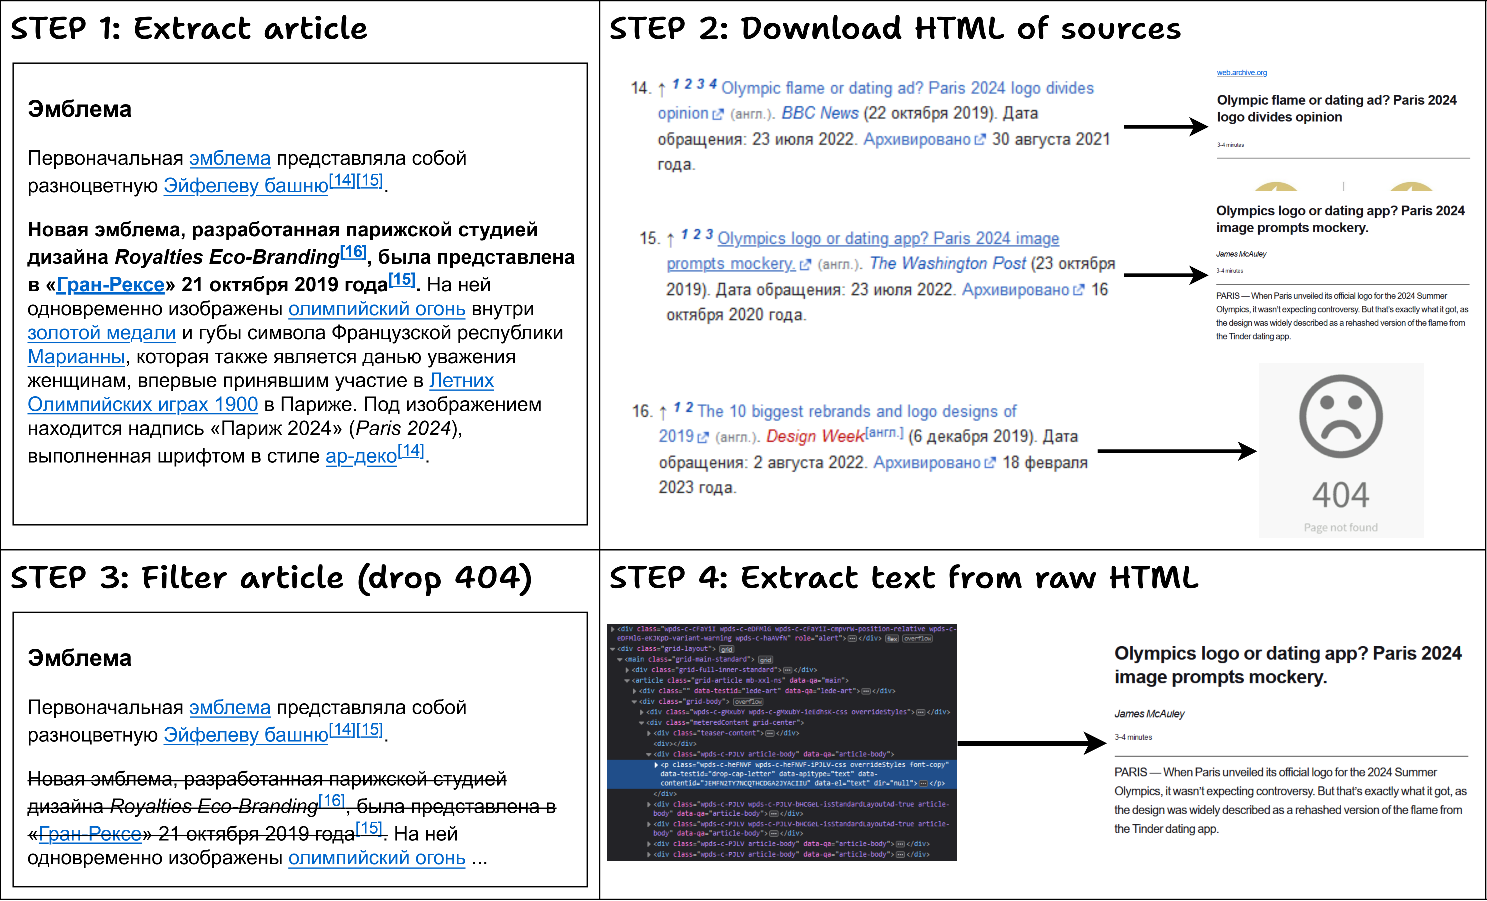
\includegraphics[width=0.6\textwidth]{figures/Source_extract.png}%
  \caption{Извлечение источников}
  \label{fig:source}
\end{figure}

\begin{figure}[htb]
  \centering
  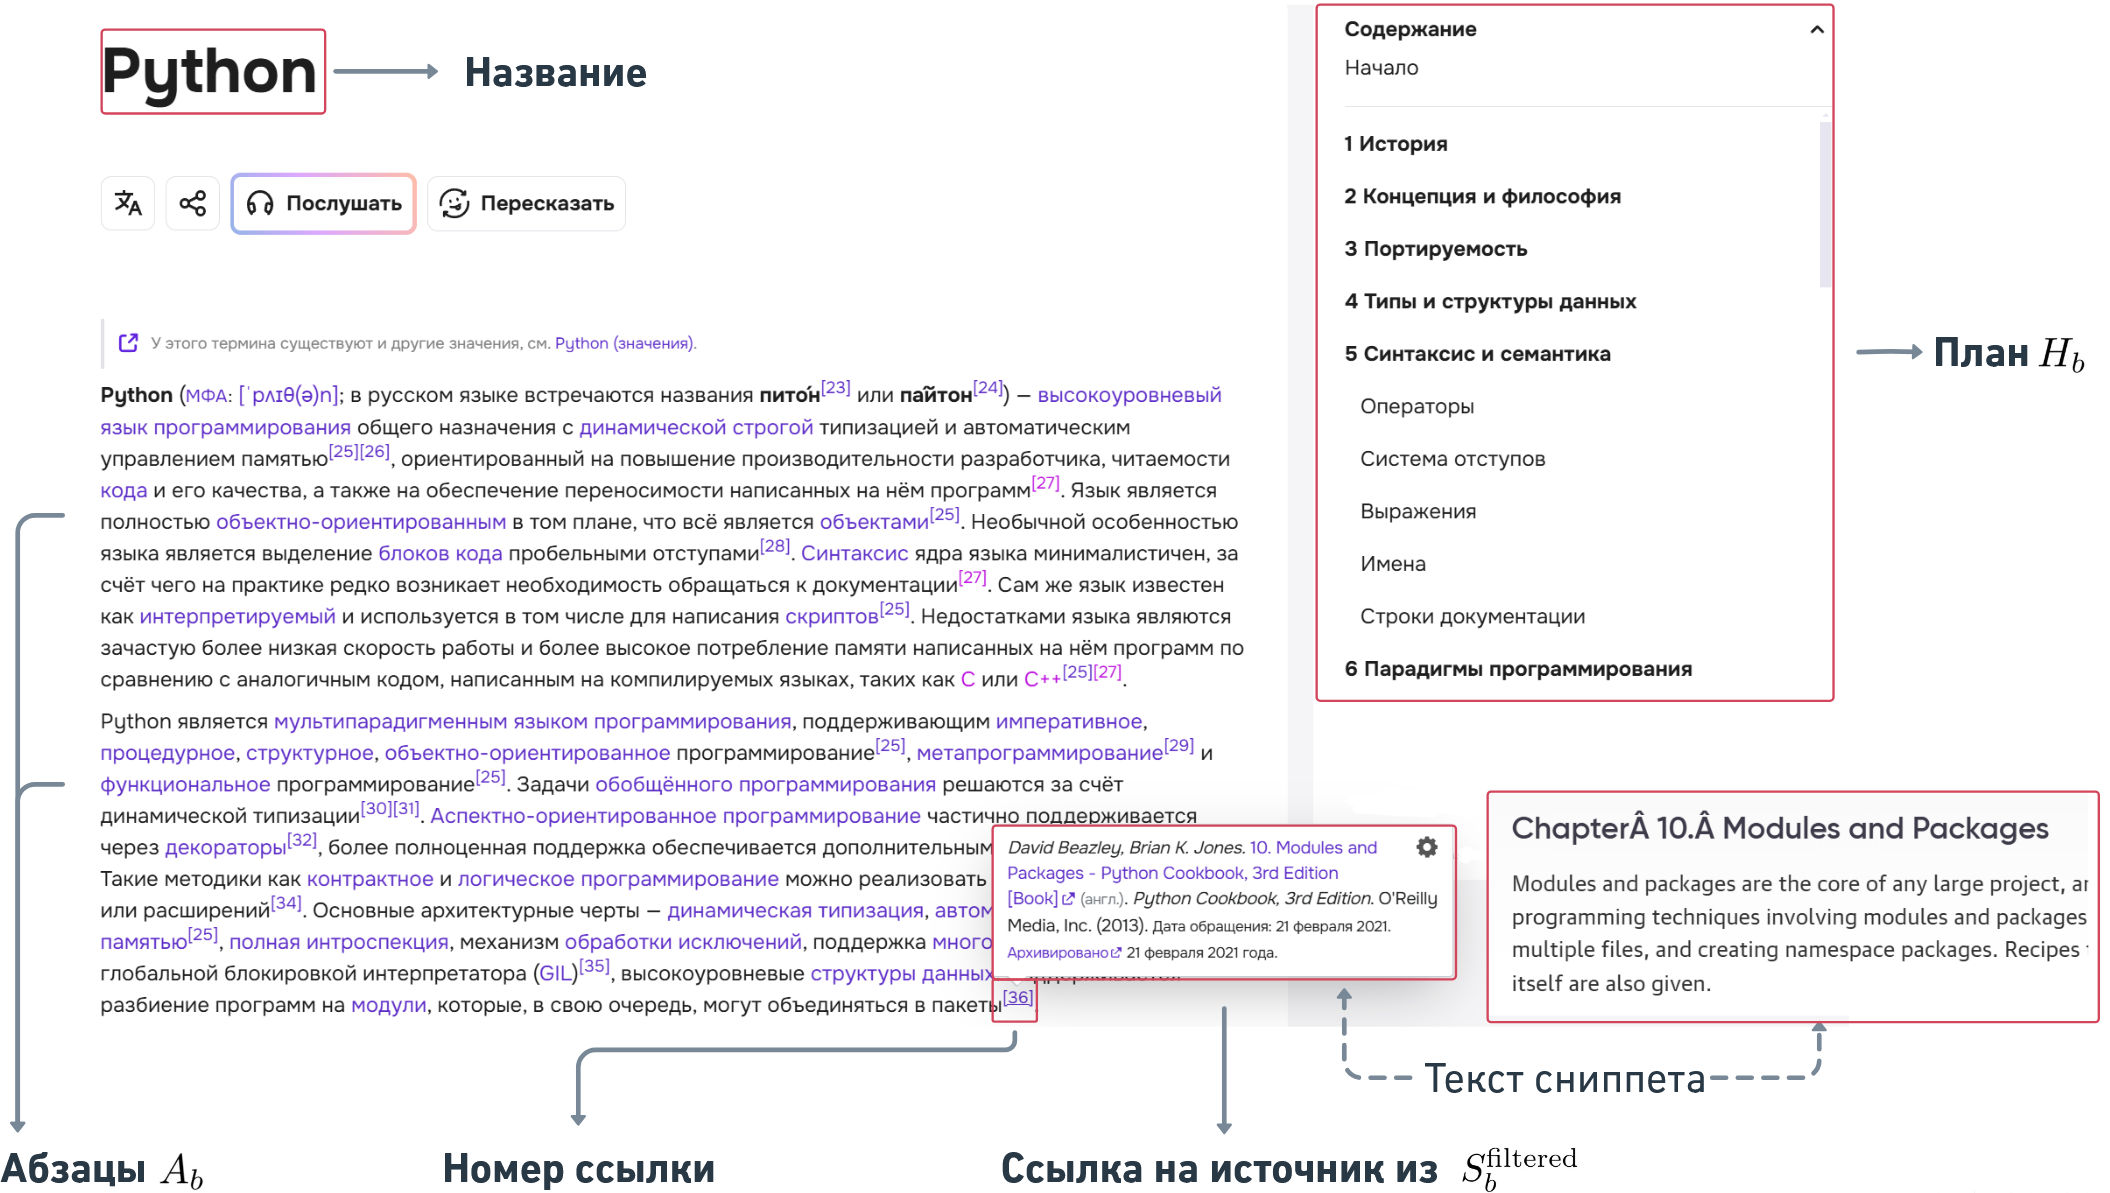
\includegraphics[width=0.6\textwidth]{figures/article_entities.png}%
  \caption{Основные сущности статьи}
  \label{fig:article}
\end{figure}

На этапе получения данных осуществляется первичное извлечение информации из выбранной статьи и сбор связанных с ней источников. 
Формально для каждой статьи \(b\in B\) задаётся её тема \(\theta_b\) и набор заголовков \(H_b=\{(h_i,l_i)\}\) с уровнями вложенности, а также набор абзацев \(A_b\) по секциям.
Извлечение HTML-кода статьи выполняется с помощью стандартных инструментов Python-модулей\footnote{https://beautiful-soup-4.readthedocs.io/en/latest/},\footnote{https://requests.readthedocs.io/en/latest/index.html}. 
Полученный текст структурируется путем разбиения на фрагменты, соответствующие вложенным заголовкам (H1, H2, H3 и т.д.), что позволяет сохранить как содержательную часть статьи, так и её иерархическую организацию. 
Далее из раздела «Примечания» автоматически извлекаются все внешние ссылки, на которые статья делает отсылки. После этого проводится проверка доступности каждой ссылки: в случае обнаружения ошибок 
(например, код 404) такие ссылки исключаются из дальнейшей обработки, а связанный с ними текст удаляется, оставляя только те источники, которые действительно доступны,
то есть источники \(S_b\) к статье фильтруются: из них выбирается подмножество \(S_b^{\mathrm{filtered}}=\{(s_q,t_q)\}\), для которых получен текст \(t_q\).
Рисунок \ref{fig:article} иллюстрирует схематичное разбиение статьи\footnote{https://ru.ruwiki.ru/wiki/Python} на ключевые сущности, используемые в дальнейшей обработке.


На этапе обработки данных выполняется фильтрация текста для обеспечения его корректной интерпретации моделью. 
Каждая сноска, обозначенная цифрами в квадратных скобках (например, [1], [2]), сопоставляется с конкретной ссылкой, соответствующей одному из доступных источников. 
То есть задано отображение \(F_b: S_b\to H_b\times A_b\), связывающее каждый источник с конкретным заголовком и абзацем.
Это позволяет точно определить позицию ссылки в тексте статьи и использовать её для последующей фильтрации. 
На основании \(S_b^{\mathrm{filtered}}\) формируются очищенные множества абзацев \(A_b^{\mathrm{filtered}}\) и заголовков \(H_b^{\mathrm{filtered}}\), 
то есть остаётся только тот контент, подкреплённый извлечёнными источниками; всё прочее удаляется. 
В результате из статьи удаляются фрагменты, опирающиеся на источники, текст которых не удалось получить, оставляя только те части текста,
которые подкреплены достоверными и доступными источниками. Характеристики собранного корпуса представлены в таблице \ref{tab:dataset}.

\begin{table}[htb]
  \centering
  \caption{Основные характеристики собранного датасета}
  \label{tab:dataset}
  \begin{tabular}{lc}
    \hline
    \textbf{Показатель} & \textbf{Значение} \\
    \hline
    Количество статей                             & 100    \\
    \hline
    Количество скачанных источников               & 5828  \\
    \hline
    Общее число сниппетов                         & 13704  \\
    \hline
    Средний размер плана (число заголовков)       & 37    \\
    \hline
    Средний размер секции (число слов)            & 112   \\
    \hline
  \end{tabular}
\end{table}


\section*{Методика оценки}
Для объективной оценки способностей языковых моделей генерировать научно-энциклопедические тексты разработана трехэтапная схема создания статьи, имитирующая реальный процесс подготовки энциклопедического контента. 
Первый этап предполагает отбор релевантных источников: модель получает заголовок статьи и набор текстовых фрагментов, среди которых необходимо идентифицировать и ранжировать по степени значимости материалы, соответствующие тематике. 
На втором этапе осуществляется построение структуры будущей статьи: на основании темы и отобранных источников модель формирует логичный план с выделением основных разделов в стиле Википедии. 
Завершающий этап посвящен непосредственной генерации текста: для каждого раздела создается связное изложение, основанное на предоставленных релевантных материалах. 

Трёхуровневая архитектура позволяет оценивать каждый аспект отдельно.
Каждому этапу соответствует специализированный набор метрик, позволяющий количественно измерить качество выполнения конкретной подзадачи. 
Такой подход не только дает разностороннюю характеристику возможностей модели, но и выявляет ее сильные и слабые стороны на разных стадиях создания научно\-популярного контента. 
Детальное описание методик оценки для каждого из этапов представлено в следующих разделах.
\subsection*{Ранжирование источников.}
Первоначально для каждой отобранной статьи на основе ее названия и всех заголовков второго уровня генерируется ее краткое описание с помощью «сильной» языковой модели. 
Описание генерируется на русском и английском языках, так как тексты источников тоже представлены в двух языковых вариантах. 
Оба варианта далее объединяются в единый текстовый запрос к системе поиска, основанной на BM25 . Так получается описание, с упомянутыми основными заголовками, как показано в Примере 1.
\begin{remark}
Статья "C++" представляет собой обзор языка программирования C++, его истории, структуры и особенностей. 
В ней рассматриваются основные аспекты языка, включая его стандартную библиотеку, отличия от языка C и дальнейшее развитие. 
Кроме того, статья содержит примеры программ на C++, сравнение с альтернативными языками программирования, а также критический анализ и обсуждение влияния C++ на развитие программирования и существующие альтернативы. 
Статья предназначена для читателей, интересующихся языком C++ и его ролью в современном программировании.
\end{remark}

Также проводились эксперименты, в которых аннотация генерировалась самими оцениваемыми моделями, опираясь только на название статьи. Краткое описание статьи, составленное только по ее названию показано в Примере 2.
\begin{remark}
Статья "C++" может быть посвящена языку программирования C++, являющимся одним из наиболее популярных и широко используемых языков программирования в мире.
В статье могут быть рассмотрены основы языка, его история, синтаксис и особенности, а также его применение в различных областях, таких как разработка операционных систем, игр и веб-приложений. 
Кроме того, статья может содержать информацию о стандартах и библиотеках C++, а также о его сравнении с другими языками программирования. 
Статья может быть полезна как для начинающих программистов, так и для опытных специалистов, которые хотят углубить свои знания о языке C++.
Статья также может включать примеры кода и практические советы по использованию C++ в реальных проектах. 
\end{remark}

В результате для каждой темы получается выдача на запрос: набор кандидатов-документов. Отобранные документы последовательно передаются большой языковой модели, которая должна определить каждый сниппет как релевантный (ответ «да») или нерелевантный (ответ «нет»). 
Для получения численных оценок и дальнейшего ранжирования берется логарифмическая вероятность токенов в ответе модели: если это был утвердительный ответ, то берется сама вероятность P(«да»), если отрицательный, то берется обратное значение, то есть 1 – P(«нет»). 
Такой подход позволяет ранжировать выдачу документов по вероятностям – то есть по уверенности модели в ответе: чем выше вероятность, тем выше степень уверенности модели в ответе, тем выше документ будет в выдаче. Полученные оценки сортируются по убыванию. 

\subsection*{Генерация плана.}

На этом этапе цель состоит в том, чтобы по множеству эталонных текстов\-источников получить полный план статьи на заданную тему.
Процесс обработки сниппетов включает несколько последовательных этапов. 
Сначала каждый текстовый фрагмент преобразуется в векторное представление с использованием выбранной модели эмбеддингов. 
Для кластеризации методом KMeans применяются предопределённые центры кластеров, соответствующие векторным представлениям документов заголовков второго уровня, причём для каждого заголовка выбирается первый документ из коллекции детерминированным способом. 
Далее отбирается 5 сниппетов, наиболее близких к центру кластера.  Формирование мини-планов секций осуществляется с учётом двух ключевых параметров: размера контекста (определяемого числом соседних сниппетов) и выбранного подхода к генерации, который может быть либо прямой генерацией по тексту документов, либо генерацией через краткое описание кластера. 
На заключительном этапе происходит объединение всех мини-планов в итоговый структурированный план статьи.

\subsection*{Генерация секций.}
На третьем и заключительном этапе формируется полный текст для каждой секции, с опорой на соответствующие документы-источники.
Все секции были предварительно отфильтрованы и содержат только тот текст, который опирается на источники, согласно сайту Рувики. 
Для каждой секции статьи извлекаются все сниппеты, которые указывались в качестве источников к данной секции. 
Это гарантирует, что модель будет генерировать текст только на основе информации соответствующих источников.  Далее все сниппеты переводятся в векторное пространство и группируются по схожести. 
Это сделано для того, чтобы избежать излишних повторов при генерации текста, например, если разные источники повторяют один и тот же текст, но немного перефразировав его. 
Для каждой такой группы формируется ее краткое описание.
Таким образом остается только некоторый набор кратких описаний – то есть была проведена фильтрация текстов и оставлена только самая важная информация и были исключены лишние повторы. 
После этого по полученным описаниям групп генерируется текст секции с использованием иерархического метода суммаризации.
\section*{Описание параметров эксперимента}

Эксперименты устроены так, чтобы из набора статей Рувики формировать ранжированную выдачу, планы и тексты на основе подкреплённого источниками контента, проходя три независимых этапа.
То есть входные данные на каждом из этапов всегда одинаковые и не зависят от других.
Ниже фиксируются все использованные данные, модели, гиперпараметры и процедуры для обеспечения воспроизводимости и анализа.

\subsection*{Данные и предобработка.}
В качестве исходного корпуса берётся подмножество статей Википедии \(B\). Для каждой статьи извлекаются заголовки (включая уровни вложенности), абзацы и указанные в них источники. 
Источники фильтруются по наличию извлечённого текста: сохраняются только те \(s_q\) из \(S_b\), для которых удалось получить текст \(t_q\) объёмом не менее 1500 символов — это условие отсекает «шумовые» ответы с HTML-страниц вроде ошибок (например, error 404) или слишком короткие фрагменты. 
Абзацы очищаются жёстко: в \(A_b^{\mathrm{filtered}}\) остаются только те абзацы, в которых присутствует хотя бы одна ссылка на источник из \(S_b^{\mathrm{filtered}}\); абзацы без ссылок или со ссылками, для которых текст не был получен, удаляются. 
Аналогично формируется \(H_b^{\mathrm{filtered}}\) — только те заголовки, под которыми остался поддерживаемый источниками текст (хотя бы один абзац).

\subsection*{Ранжирование источников.}
Для формирования запроса к поисковой системе сначала генерируется краткое описание статьи.  
В базовом варианте описание генерируется исключительно по названию статьи самой оцениваемой моделью без дополнительных заголовков.
Таким образом LLM полностью отвечает за качество выдачи и самостоятельно решает, какой поисковый запрос лучше сформулирвать для BM25.
Также проверяется и другой вариант использование «сильной» языковой модели llama3-70b: ей передаются в подсказке заголовки второго уровня текущей статьи, и по ним генерируется аннотация. 
Генерация производится на двух языках — русском и английском — для согласования с тем фактом, что тексты источников также представлены в этих вариантах. 
Оба варианта объединяются в единый текстовый запрос.

Индексирование сниппетов производится с помощью BM25 по всему корпусу собранных сниппетов без настройки гиперпараметров (стандартные значения).
Для каждого релевантного документа выбираются два нерелевантных (соотношение 1:2) — это сделано для повышения устойчивости оценки.
Выдача по запросу представляет собой набор кандидатов (сниппетов), которые последовательно передаются той же или другой большой языковой модели для классификации релевантности.
Поскольку контекстное окно маленькое, то LLM сама определяет, что будет использовать.

\subsection*{Генерация плана.}
Для планирования статьи каждый сниппет сначала переводится в векторное пространство с помощью модели эмбеддингов \texttt{sergeyzh/BERTA}. 
На основе векторных представлений происходит кластеризация методом KMeans. Число кластеров \(k\) устанавливается равным числу заголовков второго уровня исходной статьи. 
Инициализация кластеров детерминирована: для каждого заголовка в качестве начального представителя выбирается первый документ из коллекции.
Количество создаваемых кластеров $k$ соответствует числу заголовков второго уровня. 
В рамках каждого кластера $K_j$ вычисляется его центр по формуле ~\eqref{equC}:
\begin{equation}\label{equC}
\text{center}_j = \frac{1}{N_j} \sum_{e \in K_j} e
\end{equation}
В формуле ~\eqref{equC} $N_j$ обозначает количество документов в кластере $K_j$.
Из каждого кластера отбираются пять сниппетов, наиболее близких к его центру.
Формирование мини-планов секций может происходить двумя способами: напрямую по текстам этих сниппетов либо посредством предварительного генеративного описания кластера, по которому затем строится план.
Контекстное окно варьируется: используется либо нулевое окно (только сам сниппет), либо по одному соседнему сниппету слева и справа для расширения контекста. 
На финальном этапе все мини-планы объединяются в итоговый структурированный план статьи. 
В экспериментах сравниваются варианты с предварительным описанием кластера и без него, а также влияние размера окна. 

\subsection*{Генерация секций.}
На этом этапе для каждой секции извлекаются все сниппеты, ассоциированные с ней через фильтрованные источники 
(то есть только из \(A_b^{\mathrm{filtered}}\)), тем самым гарантируя, что дальнейшая генерация опирается исключительно на корректно подкреплённые ссылки. 
Все сниппеты снова переводятся в эмбеддинги и строится матрица попарных сходств как произведение \(Emb \times Emb^\top\), что по сути даёт косинусные близости между векторами. 
Элементы с значением сходства выше порога 0.8 (значение подобрано эмпирически на основании визуального анализа матрицы) считаются близкими по смыслу и объединяются в группы, 
чтобы избежать избыточных повторов при генерации (например, когда разные источники перефразируют одно и то же). 
Для каждой такой смысловой группы строится иерархическое суммарное представление: 
берутся первые \textbf{пять} текстов, по ним генерируется краткое описание, затем это описание дополняется на основе следующих пяти и так далее, пока не получено полное сжатое представление группы. 
В результате остаётся набор кратких описаний, представляющих суть схожих по содержанию фрагментов. 
Финальный текст секции генерируется с помощью иерархического метода.

\subsection*{Ресурсы.}
Все векторные вычисления и эмбеддинги вычислялись на локальной машине с GPU NVIDIA GeForce RTX 3080 Ti с объемом видеопамяти в 12 Гб.
Модель, использовавшаяся для генерации аннотаций - llama3-70b. 
Для обеспечения воспроизводимости фиксируются случайные сиды ($random\_seed = 42$). 
В коде указываются параметры обращения к LLM (temperature, max\_tokens и др.), использованные при генерации - параметры одинаковые для всех LLM, если не указано другое.


\section*{Метрики оценки качества}

В рамках бенчмарка применяются две группы метрик:  
(1) метрики ранжирования, оценивающие, насколько хорошо модель отбирает релевантные источники;  
(2) метрики текстовой схожести, измеряющие соответствие сгенерированного содержания эталонному.

\subsection*{Метрики ранжирования.}

Для оценки качества списка источников используются \textbf{NDCG@\textit{K}} и \textbf{R‑Precision}.

\begin{equation}
\mathrm{DCG@K}= \sum_{i=1}^{K} \frac{\mathrm{rel}_i}{\log_2(i+1)}\tag{3}
\end{equation}

\begin{equation}
\mathrm{IDCG@K}= \sum_{i=1}^{K} \frac{\mathrm{rel}^{\mathrm{IDEAL}}_i}{\log_2(i+1)}\tag{4}
\end{equation}

\begin{equation}
\mathrm{NDCG@K}= \frac{\mathrm{DCG@K}}{\mathrm{IDCG@K}}\tag{5}
\end{equation}

\begin{equation}
\mathrm{R\text{-}Precision}= \frac{\sum_{i=1}^{R} \mathrm{rel}_i}{R}\tag{6}
\end{equation}

В формулах \(\mathrm{rel}_i\in\{0,1\}\) — индикатор релевантности документа на позиции \(i\);  
\(\mathrm{rel}^{\mathrm{IDEAL}}_i\) — та же величина в идеальной (полностью отсортированной) выдаче;  
\(R\) — общее число релевантных документов для данного запроса.  
Нормировка через \(\mathrm{IDCG@K}\) гарантирует, что \(\mathrm{NDCG@K}\in[0,1]\), где 1 соответствует идеальному порядку.

\subsection*{Метрика текстовой схожести.}

Качество сгенерированных секций оценивается \textbf{BERTScore}, показывающим семантическое совпадение с эталоном на уровне предложений:

\begin{align}
R_{\mathrm{BERT}} &= \frac{1}{|x|}\sum_{x_i\in x}\max_{\hat{x}_j\in\hat{x}} x_i^\top \hat{x}_j\tag{7}\\
P_{\mathrm{BERT}} &= \frac{1}{|\hat{x}|}\sum_{\hat{x}_j\in\hat{x}}\max_{x_i\in x} x_i^\top \hat{x}_j\tag{8}\\
F_{\mathrm{BERT}} &= \frac{2\,P_{\mathrm{BERT}}\,R_{\mathrm{BERT}}}{P_{\mathrm{BERT}} + R_{\mathrm{BERT}}}\tag{9}
\end{align}

Здесь \(x\) — эталонный текст, \(\hat{x}\) — сгенерированный; каждое предложение кодируется эмбеддингом модели BERT, после чего вычисляется косинусное сходство.  
\(R_{\mathrm{BERT}}\) отражает полноту (recall), \(P_{\mathrm{BERT}}\) — точность (precision), а \(F_{\mathrm{BERT}}\) их гармоническое среднее.  
Значения метрики также лежат в диапазоне \([0,1]\), где 1 соответствует полному семантическому совпадению.


\section*{Описание результатов эксперимента}
Далее представлены таблицы с результатами прохождения бенчмарка некоторыми моделями. Тестирование проводилось в "дефолтном" режиме: поисковые запросы брались эталонные - сгенерированные сильной моделью по названию статьи и ее заголовкам, а
при создании плана для каждого кластера предварительно генерировалось описание.

\begin{table}[ht]
\centering
\caption{Результаты отбора источников с поиском по заранее сгенерированной аннотации}
\begin{tabular}{l|c|c}
\hline
\textbf{Model} & \textbf{nDCG} & \textbf{R‑Pr} \\
\hline
\textbf{DeepSeek V3} & \textbf{95.42} & \textbf{83.86} \\
Qwen3-235B-A22B & 94.49 & 82.42 \\
RuadaptQwen3-32B-Instruct-v2 & 95.25 & 81.81 \\
tpro & 95.42 & 83.53 \\
yagpt5lite & 90.35 & 77.66 \\
\textbf{baseline (bm25)} & \textbf{88.81} & \textbf{62.51} \\
\hline
\end{tabular}
\end{table}

Первоначально некоторые модели показывали очень низкие результаты, в связи с тем, что в выдаче проверялся именно первый сгенерированный токен. Однако не всегда модель генерирует то, что от нее просят, например может быть сгенерирован служебный
токен <think> у моделей, которые обладают способностями к размышлению. Из-за этого получаются не очень честные результаты, так как после служебного токена с наибольшей вероятностью встретится нужный. Поэтому в бенчмарке алгоритм ищет первый токен,
который совпадает либо с 'YES', либо 'NO'. Также не учитывается форматирование ответа, например лишние пробелы по бокам, что позволяет получить более достоверные результаты и не ставить низкую оценку моделям только из-за неправильного форматирования ответа.

\begin{table}[ht]
\centering
\caption{Результаты генерации заголовков}
\begin{tabular}{l|c|c}
\hline
\textbf{Model} & \textbf{Mean F1} & \textbf{[Min; Max] F1} \\
\hline
DeepSeek V3 & 65.50 & [64.82; 66.33] \\
Qwen3-235B-A22B  & 62.66 & [61.90; 63.47] \\
tpro & 60.75 & [59.89; 61.60] \\
yagpt5lite & 60.25 & [59.48; 61.00] \\
\hline
\end{tabular}
\end{table}

В бенчмарке схожесть заголовков с эталонными сравнивалась при помощи косинусной близости: учитывалось именно смысловое соответствие, а не точная формулировка или уровень заголовка. 
Сравнение проводилось с очищенной структурой статьи: из предобработанного текста удалялись все заголовки, которые полностью состояли из текста, не участвовавшего в генерации. Это позволяло честно оценить схожесть заголовков.


\begin{table}[ht]
\centering
\caption{Результаты генерации секций}
\begin{tabular}{l|c|c}
\hline
\textbf{Model} & \textbf{Mean F1} & \textbf{[Min; Max] F1} \\
\hline
DeepSeek V3 & 53.48 & [52.37; 54.85] \\
Qwen3-235B-A22B  & 53.74 & [52.56; 54.79] \\
tpro & 53.15 & [52.07; 54.50] \\
yagpt5lite & 53.43 & [52.24; 54.67] \\
\hline
\end{tabular}
\end{table}



\section*{Заключение}


\begin{thebibliography}{99}

\bibitem{resar}
\textit{ResearchArena.}
Kang H., Xiong C. ResearchArena: Benchmarking LLMs' Ability to Collect and Organize Information as Research Agents //arXiv e-prints. – 2024. – С. arXiv: 2406.10291.

\bibitem{storm}
\textit{Storm.}
Shao Y. et al. Assisting in Writing Wikipedia-like Articles From Scratch with Large Language Models //NAACL-HLT. – 2024

\bibitem{deepr}
\textit{OpenAI.}
Introducing deep research // OpenAI URL: https://openai.com/index/introducing-deep-research/ (дата обращения: 31.07.2025).

\end{thebibliography}

\renewcommand\refname{References}



\begin{thebibliography}{99}

\bibitem{resar}
\textit{ResearchArena.}
Kang H., Xiong C. ResearchArena: Benchmarking LLMs' Ability to Collect and Organize Information as Research Agents //arXiv e-prints. – 2024. – С. arXiv: 2406.10291.

\bibitem{storm}
\textit{Storm.}
Shao Y. et al. Assisting in Writing Wikipedia-like Articles From Scratch with Large Language Models //NAACL-HLT. – 2024

\bibitem{deepr}
\textit{OpenAI.}
Introducing deep research // OpenAI URL: https://openai.com/index/introducing-deep-research/ (дата обращения: 31.07.2025).

\bibitem{Lan_e}
\textit{Landau Е.}

Der Picard--Schottkysche Satz und die Blochsche Konstante //
Sitzungsber. Preuss. Akad. Wiss. Berlin, Phys.-Math. Kl. 1926. V. 32. P. 467--474.

\end{thebibliography}

\end{document}